% mnras_template.tex
%
% LaTeX template for creating an MNRAS paper
%
% v3.0 released 14 May 2015
% (version numbers match those of mnras.cls)
%
% Copyright (C) Royal Astronomical Society 2015
% Authors:
% Keith T. Smith (Royal Astronomical Society)

% Change log
%
% v3.0 May 2015
%    Renamed to match the new package name
%    Version number matches mnras.cls
%    A few minor tweaks to wording
% v1.0 September 2013
%    Beta testing only - never publicly released
%    First version: a simple (ish) template for creating an MNRAS paper

% there are 25 thermal pulses, one i am looking at is the 24th

%%%%%%%%%%%%%%%%%%%%%%%%%%%%%%%%%%%%%%%%%%%%%%%%%%
% Basic setup. Most papers should leave these options alone.
% \documentclass[a4paper,fleqn,usenatbib]{mnras}
\documentclass[fleqn,usenatbib]{mnras}

% MNRAS is set in Times font. If you don't have this installed (most LaTeX
% installations will be fine) or prefer the old Computer Modern fonts, comment
% out the following line
%\usepackage{newtxtext,newtxmath}
% Depending on your LaTeX fonts installation, you might get better results with one of these:
%\usepackage{mathptmx}
%\usepackage{txfonts}

% Use vector fonts, so it zooms properly in on-screen viewing software
% Don't change these lines unless you know what you are doing
\usepackage[T1]{fontenc}
\usepackage{ae,aecompl}
\usepackage{graphicx}


%%%%% AUTHORS - PLACE YOUR OWN PACKAGES HERE %%%%%

% Only include extra packages if you really need them. Common packages are:
\usepackage{graphicx}	% Including figure files
\usepackage{amsmath}	% Advanced maths commands
\usepackage{amssymb}	% Extra maths symbols
% macros. please check here before defining something new.
% code.tex
% LaTeX2e macros for naming codes, plus shortcuts for some common ones
% 
\newcommand{\code}[1]{\texttt{#1}}
\newcommand{\flash}{FLASH}
\newcommand{\kepler}{KEPLER}
\newcommand{\nonsmoker}{NON-SMOKER}
\newcommand{\mesa}{\code{MESA}}
\newcommand{\MESA}{\mesa}
\newcommand{\STERN}{STERN}
\newcommand{\ADIPLS}{\code{ADIPLS}}
\newcommand{\DSEP}{DSEP} 

% names for NuGrid codes and code modules
\newcommand{\mppnp}{\code{mppnp}} % multi-zone post-processing network parallel
\newcommand{\ppn}{\code{ppn}}     % refers to the whole NuGrid post-processing code family
\newcommand{\spp}{\code{spp}}     % single-zone ppn


% modules for MESA, from the original instrument paper
\newcommand{\alert}{\code{alert}}
\newcommand{\utils}{\code{utils}}
\newcommand{\const}{\code{const}}
\newcommand{\chem}{\code{chem}}
\newcommand{\diffusion}{\code{diffusion}}
\newcommand{\mtx}{\code{mtx}}
\newcommand{\mesastar}{\mesa~\code{star}}
\newcommand{\MESAstar}{\mesastar}
\newcommand{\num}{\code{num}}
\newcommand{\nuc}{\code{nuc}}
\newcommand{\kap}{\code{kap}}
\newcommand{\eos}{\code{eos}}
\newcommand{\intone}{\code{interp\_1d}}
\newcommand{\inttwo}{\code{interp\_2d}}
\newcommand{\atm}{\code{atm}}
\newcommand{\diff}{\code{diffusion}}
\newcommand{\mlt}{\code{mlt}}
\newcommand{\rates}{\code{rates}}
\newcommand{\net}{\code{net}}
\newcommand{\neu}{\code{neu}}
\newcommand{\weak}{\code{weaklib}}
\newcommand{\screen}{\code{screen}}
\newcommand{\ioniz}{\code{ionization}}
\newcommand{\adipls}{\code{adipls}}
\newcommand{\colors}{\code{colors}}
\newcommand{\reaclib}{\code{reaclib}}
\newcommand{\karo}{\code{karo}}
\newcommand{\astero}{\code{astero}}
\newcommand{\sdk}{\code{SDK}}
\newcommand{\SDK}{\sdk}

% $Id: derivatives.tex 385 2008-07-13 20:07:02Z efb $

%differential operator, roman typeface
\newcommand{\dif}{\ensuremath{\mathrm{d}}}

%derivatives
\newcommand{\D}{{\mathrm d}}
\newcommand{\DD}{{\,\D\!\!\;}}
\newcommand{\ddt}[1]{\frac{\partial #1}{\partial t}} %partial time derivative 
\newcommand{\DDt}[1]{\frac{\dif #1}{\dif t}} %total time derivative
\newcommand{\ddx}[1]{\frac{\partial #1}{\partial x}} %partial derivative wrt x 
\newcommand{\ddy}[1]{\frac{\partial #1}{\partial y}} %partial derivative wrt y 
\newcommand{\DDy}[1]{\frac{\dif #1}{\dif y}} %total derivative wrt y
\newcommand{\ddz}[1]{\frac{\partial #1}{\partial z}} %partial derivative wrt z 
\newcommand{\ppl}[2]{\left(\frac{\partial\ln #1}{\partial\ln
      #2}\right)_{\rho,T}}
\newcommand{\ppll}[2]{\left(\frac{\partial\ln #1}{\partial\ln
      #2}\right)_{\rho,T,\{X_{j\neq i}\}}}
\newcommand{\ddl}[2]{\frac{{\rm d}\ln #1}{{\rm d}\ln #2}}
\newcommand{\DxDy}[2]{{\frac{\D{#1}}{\D{#2}}}}
\newcommand{\dxdy}[2]{{\frac{\partial{#1}}{\partial{#2}}}}
\newcommand{\dxdyind}[3]{{\Brak{\frac{\D{#1}}{\D{#2}}}_{{#3}}}}
\newcommand{\dxdycz}[3]{{\Brak{\frac{\partial{#1}}{\partial{#2}}}_{{#3}}}}
%Misc
\newcommand{\Av}[1]{{\left\langle{#1}\right\rangle}}
\newcommand{\av}[1]{{\langle{#1}\rangle}}
\newcommand{\Frac}[2]{{\Brak{#1}/\Brak{#2}}}
\newcommand{\abs}[1]{{\left|{#1}\right|}}
% $Id: nuclides.tex 385 2008-07-13 20:07:02Z efb $
% nuclides.tex
% input file with macros for nuclides

% base command
\newcommand{\nuclei}[2]{\ensuremath{\mathrm{^{#1}#2}}}

% nuclides, with most highest abundance or longest half-life as default
% for example, \carbon produces ^{12}C, \carbon[13] produces ^{13}C
%
\newcommand{\neutron}{\ensuremath{n}}
\newcommand{\nt}{\neutron}
\newcommand{\proton}{\ensuremath{p}}
\newcommand{\pt}{\proton}
\newcommand{\photon}{\ensuremath{\gamma}}
\newcommand{\hydrogen}[1][1]{\nuclei{#1}{H}}
\newcommand{\helium}[1][4]{\nuclei{#1}{He}}
\newcommand{\lithium}[1][7]{\nuclei{#1}{Li}}
\newcommand{\beryllium}[1][9]{\nuclei{#1}{Be}}
\newcommand{\boron}[1][11]{\nuclei{#1}{B}}
\newcommand{\carbon}[1][12]{\nuclei{#1}{C}}
\newcommand{\nitrogen}[1][14]{\nuclei{#1}{N}}
\newcommand{\oxygen}[1][16]{\nuclei{#1}{O}}
\newcommand{\fluorine}[1][19]{\nuclei{#1}{F}}
\newcommand{\neon}[1][20]{\nuclei{#1}{Ne}}
\newcommand{\sodium}[1][23]{\nuclei{#1}{Na}}
\newcommand{\magnesium}[1][24]{\nuclei{#1}{Mg}}
\newcommand{\aluminum}[1][27]{\nuclei{#1}{Al}}
\newcommand{\silicon}[1][28]{\nuclei{#1}{Si}}
\newcommand{\phosphorus}[1][31]{\nuclei{#1}{P}}
\newcommand{\sulfur}[1][32]{\nuclei{#1}{S}}
\newcommand{\chlorine}[1][35]{\nuclei{#1}{Cl}}
\newcommand{\argon}[1][36]{\nuclei{#1}{Ar}}
\newcommand{\potassium}[1][39]{\nuclei{#1}{K}}
\newcommand{\calcium}[1][40]{\nuclei{#1}{Ca}}
\newcommand{\scandium}[1][45]{\nuclei{#1}{Sc}}
\newcommand{\titanium}[1][48]{\nuclei{#1}{Ti}}
\newcommand{\vanadium}[1][51]{\nuclei{#1}{V}}
\newcommand{\chromium}[1][52]{\nuclei{#1}{Cr}}
\newcommand{\manganese}[1][55]{\nuclei{#1}{Mn}}
\newcommand{\iron}[1][56]{\nuclei{#1}{Fe}}
\newcommand{\cobalt}[1][59]{\nuclei{#1}{Co}}
\newcommand{\nickel}[1][58]{\nuclei{#1}{Ni}}
\newcommand{\copper}[1][63]{\nuclei{#1}{Cu}}
\newcommand{\zinc}[1][64]{\nuclei{#1}{Zn}}
\newcommand{\gallium}[1][69]{\nuclei{#1}{Ga}}
\newcommand{\germanium}[1][74]{\nuclei{#1}{Ge}}
\newcommand{\arsenic}[1][75]{\nuclei{#1}{As}}
\newcommand{\selenium}[1][80]{\nuclei{#1}{Se}}
\newcommand{\bromine}[1][79]{\nuclei{#1}{Br}}
\newcommand{\krypton}[1][84]{\nuclei{#1}{Kr}}
\newcommand{\rubidium}[1][85]{\nuclei{#1}{Rb}}
\newcommand{\strontium}[1][88]{\nuclei{#1}{Sr}}
\newcommand{\yttrium}[1][89]{\nuclei{#1}{Y}}
\newcommand{\zirconium}[1][94]{\nuclei{#1}{Zr}}
\newcommand{\niobium}[1][93]{\nuclei{#1}{Nb}}
\newcommand{\molybdenum}[1][98]{\nuclei{#1}{Mo}}
\newcommand{\technetium}[1][97]{\nuclei{#1}{Tc}}
\newcommand{\ruthenium}[1][102]{\nuclei{#1}{Ru}}
\newcommand{\rhodium}[1][103]{\nuclei{#1}{Rh }}
\newcommand{\palladium}[1][106]{\nuclei{#1}{Pd}}
\newcommand{\silver}[1][107]{\nuclei{#1}{Ag}}
\newcommand{\cadmium}[1][114]{\nuclei{#1}{Cd}}
\newcommand{\indium}[1][115]{\nuclei{#1}{In}}
\newcommand{\tin}[1][120]{\nuclei{#1}{Sn}}
\newcommand{\antimony}[1][121]{\nuclei{#1}{Sb}}
\newcommand{\tellurium}[1][130]{\nuclei{#1}{Te}}
\newcommand{\iodine}[1][127]{\nuclei{#1}{I}}
\newcommand{\xenon}[1][132]{\nuclei{#1}{Xe}}
\newcommand{\cesium}[1][133]{\nuclei{#1}{Cs}}
\newcommand{\barium}[1][138]{\nuclei{#1}{Ba}}
\newcommand{\lanthanum}[1][139]{\nuclei{#1}{La}}
\newcommand{\cerium}[1][140]{\nuclei{#1}{Ce}}
\newcommand{\praseodymium}[1][141]{\nuclei{#1}{Pr}}
\newcommand{\neodymium}[1][142]{\nuclei{#1}{Nd}}
\newcommand{\promethium}[1][147]{\nuclei{#1}{Pm}}
\newcommand{\samarium}[1][152]{\nuclei{#1}{Sm}}
\newcommand{\europium}[1][153]{\nuclei{#1}{Eu}}
\newcommand{\gadolinium}[1][158]{\nuclei{#1}{Gd}}
\newcommand{\terbium}[1][159]{\nuclei{#1}{Tb}}
\newcommand{\dysprosium}[1][164]{\nuclei{#1}{Dy}}
\newcommand{\holmium}[1][165]{\nuclei{#1}{Ho}}
\newcommand{\erbium}[1][168]{\nuclei{#1}{Er}}
\newcommand{\thulium}[1][169]{\nuclei{#1}{Tm}}
\newcommand{\ytterbium}[1][174]{\nuclei{#1}{Yb}}
\newcommand{\lutetium}[1][175]{\nuclei{#1}{Lu}}
\newcommand{\hafnium}[1][180]{\nuclei{#1}{Hf}}
\newcommand{\tantalum}[1][180]{\nuclei{#1}{Ta}}
\newcommand{\tungsten}[1][184]{\nuclei{#1}{W}}
\newcommand{\rhenium}[1][187]{\nuclei{#1}{Re}}
\newcommand{\osmium}[1][192]{\nuclei{#1}{Os}}
\newcommand{\iridium}[1][193]{\nuclei{#1}{Ir}}
\newcommand{\platnium}[1][195]{\nuclei{#1}{Pt}}
\newcommand{\gold}[1][197]{\nuclei{#1}{Au}}
\newcommand{\mercury}[1][202]{\nuclei{#1}{Hg}}
\newcommand{\thallium}[1][205]{\nuclei{#1}{Tl}}
\newcommand{\lead}[1][208]{\nuclei{#1}{Pb}}
\newcommand{\bisumth}[1][209]{\nuclei{#1}{Bi}}
\newcommand{\polonium}[1][210]{\nuclei{#1}{Po}}
\newcommand{\astatine}[1][210]{\nuclei{#1}{At}}
\newcommand{\radon}[1][222]{\nuclei{#1}{Rn}}
\newcommand{\francium}[1][223]{\nuclei{#1}{Fr}}
\newcommand{\radium}[1][226]{\nuclei{#1}{Ra}}
\newcommand{\actinium}[1][227]{\nuclei{#1}{Ac}}
\newcommand{\thorium}[1][232]{\nuclei{#1}{Th}}
\newcommand{\protactinium}[1][231]{\nuclei{#1}{Pa}}
\newcommand{\uranium}[1][238]{\nuclei{#1}{U}}
\newcommand{\neptunium}[1][237]{\nuclei{#1}{Np}}
\newcommand{\plutonium}[1][244]{\nuclei{#1}{Pu}}
\newcommand{\americium}[1][243]{\nuclei{#1}{Am}}
\newcommand{\curium}[1][247]{\nuclei{#1}{Cm}}
\newcommand{\berkelium}[1][247]{\nuclei{#1}{Bk}}
\newcommand{\californium}[1][251]{\nuclei{#1}{Cf}}
\newcommand{\einsteinium}[1][252]{\nuclei{#1}{Es}}
\newcommand{\fermium}[1][257]{\nuclei{#1}{Fm}}
\newcommand{\mendelevium}[1][258]{\nuclei{#1}{Md}}
\newcommand{\nobelium}[1][259]{\nuclei{#1}{No}}
\newcommand{\lawrencium}[1][262]{\nuclei{#1}{Lr}}
\newcommand{\rutherfordium}[1][261]{\nuclei{#1}{Rf}}
\newcommand{\dubnium}[1][268]{\nuclei{#1}{Db}}
\newcommand{\seaborgium}[1][271]{\nuclei{#1}{Sg}}
\newcommand{\bohrium}[1][274]{\nuclei{#1}{Bh}}
\newcommand{\hassium}[1][270]{\nuclei{#1}{Hs}}
\newcommand{\meitnerium}[1][278]{\nuclei{#1}{Mt}}
\newcommand{\darmstadtium}[1][281]{\nuclei{#1}{Ds}}
\newcommand{\roentgenium}[1][281]{\nuclei{#1}{Rg}}
\newcommand{\copernicum}[1][285]{\nuclei{#1}{Cn}}

\newcommand{\pdcz}{pulse-driven convective zone}

\newcommand{\spr}{\mbox{$s$-process}}
\newcommand{\sprn}{\mbox{$s$ process}}
\newcommand{\ipr}{\mbox{$i$-process}}
\newcommand{\iprn}{\mbox{$i$ process}}
\newcommand{\npr}{\mbox{$n$-process}}
\newcommand{\nprn}{\mbox{$n$ process}}
\newcommand{\rpr}{\mbox{$r$-process}}
\newcommand{\rprn}{\mbox{$r$ process}}
\newcommand{\ppr}{\mbox{$p$-process}}
\newcommand{\pprn}{\mbox{$p$ process}}

% $Id: units.tex 385 2008-07-13 20:07:02Z efb $

%------------------------------------------------------------------------
% typesetting of units
% 
% Note that this doesn't prevent linebreaking between symbol and unit.
% A more sophisticated system is available from CTAN asa units.sty
%------------------------------------------------------------------------

% basic unit typesetteing
\newcommand{\unitspace}{\ensuremath{\,}}
\newcommand{\usp}{\unitspace}
\newcommand{\numberspace}{\ensuremath{\;}}
\newcommand{\nsp}{\numberspace}
\newcommand{\unitstyle}[1]{\ensuremath{\mathrm{#1}}}
\newcommand{\power}[2]{\ensuremath{{#1}^{#2}}}
\newcommand{\natlog}[2]{\ensuremath{#1\times 10^{#2}}} % a*10^b   
\newcommand{\ee}[1]{\ensuremath{\times 10^{#1}}}

% prefixes
\newcommand{\nano}{\unitstyle{n}}
\newcommand{\milli}{\unitstyle{m}}
\newcommand{\centi}{\unitstyle{c}}
\newcommand{\kilo}{\unitstyle{k}}
\newcommand{\Mega}{\unitstyle{M}}
\newcommand{\Giga}{\unitstyle{G}}

% base units, mks
\newcommand{\meter}{\unitstyle{m}}
\newcommand{\kilogram}{\kilo\gram}
\newcommand{\second}{\unitstyle{s}}

\newcommand{\Kelvin}{\unitstyle{K}}
\newcommand{\K}{\Kelvin}  %degrees Kelvin

% base units, cgs
\newcommand{\cm}{\centi\meter}
\newcommand{\gram}{\unitstyle{g}}

% derived units
\newcommand{\grampercc}{\gram\usp\power{\cm}{-3}} %mass density
\newcommand{\grampersquarecm}{\gram\usp\power{\cm}{-2}} %column depth
\newcommand{\squarecmpergram}{\power{\cm}{2}\usp\power{\gram}{-1}} %opacity
\newcommand{\GramPerCc}{\grampercc}
\newcommand{\GramPerSc}{\grampersquarecm}
\newcommand{\columnunit}{\grampersquarecm}
\newcommand{\dyne}{\unitstyle{dyn}} %dyne
\newcommand{\erg}{\unitstyle{ergs}} %ergs
\newcommand{\ergs}{\erg}
\newcommand{\gauss}{\unitstyle{G}} %gauss
\newcommand{\ergspersecond}{\erg\unitspace\power{\second}{-1}}
\newcommand{\ergspergram}{\erg\unitspace\power{\gram}{-1}}
\newcommand{\ergspergs}{\erg\unitspace\power{\gram}{-1}\unitspace\power{\second}{-1}} %angular momentum
\newcommand{\ergssecond}{\erg\unitspace\second}
\newcommand{\cgsflux}{\erg\unitspace\power{\cm}{-2}\usp\power{\second}{-1}}

% Nuclear and atomic units
\newcommand{\amu}{\unitstyle{u}} %atomic mass unit
\newcommand{\angstrom}{\mbox{\AA}} %Angstrom
\newcommand{\fermi}{\unitstyle{fm}} %fermi
\newcommand{\eV}{\unitstyle{eV}}        %eV
\newcommand{\keV}{\kilo\eV} %Kev
\newcommand{\MeV}{\Mega\eV} %MeV

% solar and astronomical units
\newcommand{\Msun}{\ensuremath{\unitstyle{M}_\odot}}
\newcommand{\Lsun}{\ensuremath{\unitstyle{L}_{\odot}}}
\newcommand{\Rsun}{\ensuremath{\unitstyle{R}_{\odot}}}
\newcommand{\Zsun}{\ensuremath{Z_{\odot}}}
\newcommand{\Myr}{\Mega\yr}
\newcommand{\Gyr}{\Giga\yr}
\newcommand{\parsec}{\unitstyle{pc}}
\newcommand{\kpc}{\kilo\parsec} %kiloparsec
\newcommand{\mJy}{\unitstyle{\mu Jy}} %micro Jansky
\newcommand{\Msunyr}{\Msun\,\power{\yr}{-1}}
\newcommand{\MJ}{\ensuremath{\mathrm{M_J}}}
\newcommand{\RJ}{\ensuremath{\mathrm{R_J}}}
\newcommand{\AU}{\unitstyle{AU}}

% misc. units
\newcommand{\minute}{\unitstyle{min}} %minute
\newcommand{\hour}{\unitstyle{hr}} %hour
\newcommand{\yr}{\unitstyle{yr}}        %year
\newcommand{\km}{\kilo\meter}   %kilometers
\newcommand{\Hz}{\unitstyle{Hz}}        %Hertz
\newcommand{\ksec}{\kilo\second} %kilosecond
\newcommand{\kms}{\ensuremath{\mathrm{km}\,\second^{-1}}\xspace}
\newcommand{\vcrit}{{\varv_{\mathrm{crit}}}}
\newcommand{\vkep}{{\varv_{\mathrm{kep}}}}
\newcommand{\vsurf}{{\varv_{\mathrm{surf}}}}
\newcommand{\mol}{\unitstyle{mol}}% mole
\newcommand{\barn}{\unitstyle{b}} %barn

% command to include values
\newcommand{\unit}[2]{\ensuremath{#1\numberspace\mathrm{#2}}}

%=======================================================================
%
% vectors.tex---some basic vector operators
%
% Requires package bm.sty
%
%=======================================================================

\RequirePackage{bm}
%\RequirePackage{amssymb}
%\RequirePackage{amsbsy}
\newcommand{\bvec}[1]{\ensuremath{\boldsymbol{#1}}} %boldface vector style
\newcommand{\grad}{\bvec{\nabla}} %gradient
\newcommand{\divr}{\nabla \cdot} %divergence
\newcommand{\curl}{\bvec{\nabla \times}} %curl
\newcommand{\lap}{\ensuremath{\nabla^2}} %Laplacian
\newcommand{\btens}[1]{\ensuremath{\boldsymbol{\mathsf{#1}}}}
\newcommand{\vcross}{\bvec{\times}}
\newcommand{\vdot}{\bvec{\cdot}}
% end vectors.tex

%=======================================================================
%
% formatting.tex --- Formatting Macros
%
%=======================================================================

%References

\newcommand{\lSect}[1]{{\label{sec:#1}}}
\newcommand{\lFig}[1]{{\label{fig:#1}}}
\newcommand{\lEq}[1]{{\label{eq:#1}}}
\newcommand{\lTab}[1]{{\label{tab:#1}}}
\newcommand{\pFig}[1]{{\placefigure{fig:#1}}}
\newcommand{\pTab}[1]{{\placetable{tab:#1}}}
\newcommand{\Tabff}[1]{{\ref{tab:#1}}}
\newcommand{\Tab}[1]{{Table~\Tabff{#1}}}
\newcommand{\Tabs}[1]{{Tables~\Tabff{#1}}}
\newcommand{\TabRange}[2]{{Tables~\Tabff{#1} - \Tabff{#2}}}
\newcommand{\TabTwo}[2]{{Tables~\Tabff{#1} and \Tabff{#2}}}
\newcommand{\pan}[1]{{\textit{#1}}}
\newcommand{\Pan}[1]{{Panel~\pan{#1}}}
\newcommand{\Pans}[1]{{Panels~\pan{#1}}}
\newcommand{\FIGFF}[2]{{\ref{fig:#2}\pan{#1}}}
\newcommand{\Figff}[1]{{\FIGFF{}{#1}}}
\newcommand{\FIG}[2]{{Fig.~\FIGFF{#1}{#2}}}
\newcommand{\Fig}[1]{{\FIG{}{#1}}}
\newcommand{\FigTwo}[2]{{\FIGS{}{#1} and \FIGFF{}{#2}}}
\newcommand{\FIGS}[2]{{Figs.~\FIGFF{#1}{#2}}}
\newcommand{\Figs}[1]{{\FIGS{}{#1}}}
\newcommand{\Figure}[1]{{Figure~\FIGFF{}{#1}}}
\newcommand{\Figures}[1]{{Figures~\FIGFF{}{#1}}}
\newcommand{\Sectff}[1]{{\ref{sec:#1}}}
\newcommand{\Sect}[1]{{\S\Sectff{#1}}}
\newcommand{\Appendix}[1]{{Appendix~\Sectff{#1}}}
\newcommand{\Appendices}[1]{{Appendices~\Sectff{#1}}}
\newcommand{\Sects}[1]{{\S\S\Sectff{#1}}}
\newcommand{\Eqref}[1]{{\ref{eq:#1}}}
\newcommand{\Eqff}[1]{{(\Eqref{#1})}}
\newcommand{\EQ}[1]{{Equation~\Eqff{#1}}}
\newcommand{\Equation}[1]{{Equation~\Eqff{#1}}}
\newcommand{\Eq}[1]{{Eq.~\Eqff{#1}}}
\newcommand{\Eqs}[1]{{Eqs.~\Eqff{#1}}}
\newcommand{\Leg}[1]{{\textit{#1}}}

% formatting macros

\newcommand{\isofont}[1]{{\mathrm{#1}}}
\newcommand{\isomass}[1]{{\ensuremath{\isofont{^{#1}}}}}
\newcommand{\isocharge}[1]{{\ensuremath{\isofont{_{#1}}}}}
\newcommand{\isotope}[3]{{\ensuremath{\isocharge{#1}\isomass{#2}\isofont{#3}}}}
\newcommand{\Solar}[1]{{\ensuremath{\left[\right.}#1\ensuremath{\right.\left]}}}
\newcommand{\I}[2]{{\isotope{}{#1}{#2}}}
\newcommand{\El}[1]{{\I{}{#1}}}
\newcommand{\Rat}[4]{{\I{#1}{#2}/\I{#3}{#4}}}
\newcommand{\SolRatI}[4]{{\Solar{\Rat{#1}{#2}{#3}{#4}}}}
\newcommand{\SolI}[2]{{\Solar{\I{#1}{#2}}}} \newcommand{\SolEl}[1]{{\Solar{\El{#1}}}} 
\newcommand{\Ep}[1]{{\ensuremath{10^{#1}}}}
\newcommand{\E}[1]{{\ensuremath{\powersep\Ep{#1}}}}
\newcommand{\EE}[2]{{\ensuremath{\powersep\Ep{#1#2}}}}
\newcommand{\powersep}{\times}
\newcommand{\Brak}[1]{{\left({#1}\right)}}
\newcommand{\SBrak}[1]{{\left[{#1}\right]}}
\newcommand{\mem}[1]{\ensuremath{\mathrm{ #1}}}

% symbols for commonly used expressions in the paper.  The point is to define these for 
% consistent notation.  Before defining or using an expression, check that someone hasn't defined it already.
\newcommand{\epsnuc}{\ensuremath{\epsilon_{\mathrm{nuc}}}}	% nuclear heating rate
\newcommand{\epsgrav}{\ensuremath{\epsilon_{\mathrm{grav}}}} % gravitational heating rate
\newcommand{\epsnu}{\ensuremath{\epsilon_{\mathrm{\nu}}}} % neutrino losses
\newcommand{\Teff}{\ensuremath{T_{\!\mathrm{eff}}}}	% effective temperature
\newcommand{\teff}{\Teff}
\newcommand{\Ledd}{\ensuremath{L_{\mathrm{Edd}}}} % Eddington Luminosity
\newcommand{\logg}{\ensuremath{\log g}}	% log surface gravity
\newcommand{\Tc}{\ensuremath{T_{\mathrm{\!c}}}} % central temperature
\newcommand{\Pc}{\ensuremath{P_{\mathrm{\!c}}}} % central pressure
\newcommand{\rhoc}{\ensuremath{\rho_{\mathrm{c}}}} % central density
\newcommand{\CP}{\ensuremath{C_{\!P}}} % specific heat at constant pressure
\newcommand{\Mdot}{\ensuremath{\dot{M}}} % mass-loss rate
\newcommand{\Mc}{\ensuremath{M_{\rm c}}} % core mass
\newcommand{\Mm}{\ensuremath{M_{\rm m}}} % modeled mass
\newcommand{\Rc}{\ensuremath{R_{\rm c}}} % core radius
\newcommand{\Lc}{\ensuremath{L_{\rm c}}} % core luminosity
\newcommand{\Lacc}{\ensuremath{L_{\rm acc}}} % accretion luminosity

% opacity stuff
\newcommand{\kappath}{\ensuremath{\kappa_{\mathrm{th}}}} % opacity for thermal radiation orig.\ in planet
\newcommand{\kappav}{\ensuremath{\kappa_{\mathrm{v}}}} % opacity for irradiation from star

% for correction between baryon densities and mass-energy densities
\newcommand{\nB}{\ensuremath{n_{\mathrm{B}}}}	% baryon density
%
% symbols from the first instrument paper
\newcommand{\alphaMLT}{\ensuremath{\alpha_{\mathrm{MLT}}}}	% mixing length parameter
\newcommand{\chirho}{\ensuremath{\chi_{\rho}}}	% $(\partial\ln P/\partial\ln\rho)_T$
\newcommand{\chiT}{\ensuremath{\chi_{\raisebox{-2pt}{$\scriptstyle T$}}}}	% $(\partial\ln P/\partial\ln T)_{\rho}$
\newcommand{\Gammaone}{\ensuremath{\Gamma_{\!1}}} % $ (\partial\ln P/\partial \ln\rho)_S$
\newcommand{\Dov}{\ensuremath{D_{\mathrm{ov}}}}	% overshoot diffusion coefficient
\newcommand{\nablaad}{\ensuremath{\nabla_{\!\mathrm{ad}}}}	% adiabatic temperature gradient
\newcommand{\nablarad}{\ensuremath{\nabla_{\!\mathrm{rad}}}}	% radiative temperature gradient
\newcommand{\nablaT}{\ensuremath{\nabla_{\!T}}}	% actual temperature gradient
\newcommand{\nablaL}{\ensuremath{\nabla_{\mathrm{\!L}}}}	% Ledoux criterion
\newcommand{\scaleheight}{\ensuremath{\lambda_P}}	% pressure scale height
\newcommand{\Pgas}{\ensuremath{P_{\!\!\mathrm{gas}}}}	% gas pressure
\newcommand{\timestep}{\ensuremath{\delta t}} % numerical timestep
%
% more symbols for radiation and gas pressures
\newcommand{\Prad}{\ensuremath{P_{\!\!\mathrm{rad}}}}	% radiation pressure
\newcommand{\Lrad}{\ensuremath{L_{\mathrm{rad}}}}	% radiative luminosity
\newcommand{\tderiv}[3]{\ensuremath{\left(\frac{\partial #1}{\partial #2}\right)_{#3}}} %thermodynamic derivative
\newcommand{\Lrho}{\ensuremath{L_{\mathrm{inv}}}}	% luminosity at which a density inversion occurs
\newcommand{\Lonset}{\ensuremath{L_{\mathrm{onset}}}}	% luminosity at which the onset of convection occurs
\newcommand{\Fconv}{\ensuremath{F_{\!\mathrm{conv}}}}		% convective flux
\newcommand{\Frad}{\ensuremath{F_{\!\mathrm{rad}}}}	% radiative flux
\newcommand{\supernab}{\ensuremath{\delta_\nabla}}  % superadiabaticity, $\nablaT-\nablaad$
\newcommand{\superthresh}{\ensuremath{\delta_{\nabla,\mathrm{thresh}}}}  % controls when MLT++ is applied
\newcommand{\fsuper}{\ensuremath{f_\nabla}} % reduction factor for $\supernab$
\newcommand{\asuper}{\ensuremath{\alpha_\nabla}}  % smoothing parameter for MLT++
\newcommand{\asupert}{\ensuremath{\widetilde{\asuper}}} % MLT++ parameter used in construction of \asuper
\newcommand{\lambdamax}{\ensuremath{\lambda_{\max}}} % $ \max(\Lrad/\Ledd)$
\newcommand{\betamin}{\ensuremath{\beta_{\min}}} % $ \min(P/\Pgas)$

% mixing symbols
\newcommand{\alphasc}{\ensuremath{\alpha_{\mathrm{sc}}}} % semiconvection efficiency parameter
\newcommand{\alphath}{\ensuremath{\alpha_{\mathrm{th}}}} % thermohaline efficiency parameter
\newcommand{\Dth}{\ensuremath{D_{\mathrm{th}}}} % thermohaline diffusion coefficient

\newcommand{\EFc}{\ensuremath{E_{\mathrm{F,c}}}}  % Fermi energy at center
%
% physical constants
\newcommand{\kB}{\ensuremath{k_\mathrm{B}}} % Boltzmann constant
\newcommand{\NA}{\ensuremath{N_\mathrm{\!A}}} % Avogadro number
\newcommand{\mb}{\ensuremath{m_\mathrm{u}}} % atomic mass unit
\newcommand{\sigmaSB}{\ensuremath{\sigma_\mathrm{\!SB}}} % Stefan-Boltzmann constant

% rotation
\newcommand{\veq}{\ensuremath{\varv_{\mathrm{eq}}}} % equatorial velocity
\newcommand{\veqi}{\ensuremath{\varv_{\mathrm{eq,ini}}}}
\newcommand{\Om}{\ensuremath{\Omega}}  % surface angular velocity
\newcommand{\Omc}{\ensuremath{\Om_{\mathrm{crit}}}} % surface critical angular velocity
\newcommand{\om}{\ensuremath{\omega}}  %  angular velocity
\newcommand{\tkh}{\ensuremath{\tau_{\mathrm{KH}}}} % thermal (Kelvin-Helmholtz) timescale
\newcommand{\LP}{{L_{\mathrm{P}}}} 
\newcommand{\VP}{{V_{\mathrm{P}}}}
\newcommand{\SP}{{S_{\!\mathrm{P}}}} 
\newcommand{\rP}{{r_{\mathrm{P}}}}
\newcommand{\mP}{{m_{\mathrm{P}}}} 
\newcommand{\fP}{{f_{\mathrm{P}}}}
\newcommand{\fT}{{f_{\mathrm{T}}}}

% asteroseismology
\newcommand{\numax}{\ensuremath{\nu_{\mathrm{max}}}} % frequency of maximum power
\newcommand{\dnu}{\ensuremath{\Delta\nu}}  % large frequency separation of pulsation modes
\newcommand{\fov}{\ensuremath{f_{\mathrm{ov}}}} % convective overshoot parameter
\newcommand{\cs}{\ensuremath{c_{\rm s}}} % adiabatic sound speed
\newcommand{\Slamb}{\ensuremath{S_{\!\ell}}} % Lamb frequency


%%%%% AUTHORS - PLACE YOUR OWN COMMANDS HERE %%%%%
% misc. abbreviations
\newcommand{\paperone}{Paper~I} % the first paper

% Please keep new commands to a minimum, and use \newcommand not \def to avoid
% overwriting existing commands. Example:
\newcommand{\pcm}{\,cm$^{-2}$}	% per cm-squared

%%%%%%%%%%%%%%%%%%%%%%%%%%%%%%%%%%%%%%%%%%%%%%%%%%


%%%%%%%%%%%%%%%%%%%%%%%%%%%%%%%%%%%%%%%%%%%%%%%%%%

%% NuGrid/MESA way
%%
% see https://en.wikibooks.org/wiki/LaTeX/Colors for selection of
% colors, such as Apricot Aquamarine BlueGreen BurntOrange
% CornflowerBlue Emerald Gray Lavender Maroon NavyBlue Orchid Plum Red
% RoyalBlue SeaGreen Tan Violet YellowOrange

% for comments
\newcommand{\shortcomment}[3]{\textcolor{#1}{[#2: #3]}}
% for the Ready-To-Read sign off
\newcommand{\rtr}[1]{\shortcomment{red}{RTR}{#1}}
% for freezing a section
\newcommand{\sectionisfrozen}[1]{\textcolor{BlueViolet}{\textsf{\bfseries[section is frozen: send comments to #1]}}}
\newcommand{\sectionisdone}{\textcolor{Green}{\textsf{\bfseries[section is done]}}}

% if you want to embed comments in the text, clone the following with
% a color and your initials...

% for author's comments; choose your own color and replace 'fh' and
% 'FH' with your name and initials
\newcommand{\fhcom}[1]{\shortcomment{PineGreen}{FH}{#1}}

%%%%%%%%%%%%%%%%%%% TITLE PAGE %%%%%%%%%%%%%%%%%%%

% Title of the paper, and the short title which is used in the headers.
% Keep the title short and informative.
\title[Nucleosynthesis in a 2\Msun He-Flash Pulse Driven Convection Zone]{Nucleosynthesis in a 2M$_{\odot}$ He-Flash Pulse Driven Convection Zone}

% The list of authors, and the short list which is used in the headers.
% If you need two or more lines of authors, add an extra line using \newauthor
\author[D. Stephens]{
David Stephens}


% These dates will be filled out by the publisher
%\date{Accepted XXX. Received YYY; in original form ZZZ}

% Enter the current year, for the copyright statements etc.
%\pubyear{2015}

% Don't change these lines
\begin{document}
\label{firstpage}
\pagerange{\pageref{firstpage}--\pageref{lastpage}}
\maketitle

% Abstract of the paper
\begin{abstract}
During the asymptotic giant branch (AGB) phase of stellar evolution for a 2\Msun, $Z=0.02$ star, the periodic thermal pulses form a \carbon[13] pocket which can start the \spr~from the \carbon[13]($\alpha,n$)\oxygen[16] reaction. Soon after, the He-flash causes a convection zone to form with temperatures as high as 2.9\ee{8} \K~and mixes the contents of the \carbon[13] pocket. With these temperatures, the \neon[22]($\alpha,n$)\magnesium[25] reaction is activated which leads to a second start of the \spr~and this readjusts the isotopic per mil ratio of \zirconium[96] and \zirconium[94], $\delta$(\zirconium[96] / \zirconium[94]), due to neutron densities reaching as high as 1\ee{10} \power{\centi\meter}{-3}. With a modified diffusion coefficient characterized by 3D hydrodynamic stellar convection simulations, the nucleosynthetic impacts at this stage of evolution are described. Of particular interest are the impacts this has for the branching at \zirconium[95] and \iodine[128]. The changes to the diffusion coefficient adjust the $\delta$(\zirconium[96] / \zirconium[94]) to better match the observed $\delta$(\zirconium[96] / \zirconium[94]) measured from pre-solar SiC grains.
\end{abstract}

% Select between one and six entries from the list of approved keywords.
% Don't make up new ones.
\begin{keywords}
AGB -- Convection -- Nucleosynthesis -- Pre-solar SiC Grains
\end{keywords}

%%%%%%%%%%%%%%%%%%%%%%%%%%%%%%%%%%%%%%%%%%%%%%%%%%

%%%%%%%%%%%%%%%%% BODY OF PAPER %%%%%%%%%%%%%%%%%%

\section{Introduction}

The Zr isotopes are produced from the \spr~within stars and \iron[56] is the seed. To start the \spr~the neutron densities must reach above 1\ee{8}  \power{\centi\meter}{-3} and in order to affect the Zr isotopes it must pass the first peak at \strontium[88]. One of the \spr~sites in middle mass stars is during the thermal pulses caused by successive He-flashes in their asymptotic giant branch (AGB) phase. In between these thermal pulses the \carbon[13] pocket develops and through the \carbon[13]($\alpha,n$)\oxygen[16] reaction the \spr~pccurs. Then, this material will be mixed into the He-flash pulse driven convection zone (PDCZ) and the \neon[22]($\alpha,n$)\magnesium[25] reaction will activate the \spr~again for a few years. The neutron densities that are achieved through these two processes differs significantly and depends on the conditions in the star. The Zr isotopic ratios can be used to understand the conditions within the AGB stars as they are sensitive to the neutron densities that they are exposed to \citep{zr}.

The \zirconium[95] isotope is unstable with a lifetime of 64 days. Within the \carbon[13] pocket, the neutron densities do not get large enough to allow for the \zirconium[95] branch to open so most of the \zirconium[95] will decay to \molybdenum[95] rather than undergo the neutron capture \zirconium[95]($n,\gamma$)\zirconium[96]. This skews the isotopic ratios of \zirconium[96] / \zirconium[94] as there will be production of \zirconium[94] but almost none of \zirconium[96] during the \spr~within the \carbon[13] pocket. However, once the He-flash PDCZ forms, the \neon[22]($\alpha,n$)\magnesium[25] reaction can generate neutron densities as large as 1\ee{10} \power{\centi\meter}{-3} which will open the branch for the \zirconium[95]($n,\gamma$)\zirconium[96] to occur, shifting the isotopic ratios again. Many of these thermal pulses happen throughout the AGB phase and some of the material left behind from the He-flash PDCZ can be mixed into the H envelope by the third dredge up that occurs after each thermal pulse. Due to the significant mass loss during the AGB phase, the isotopic ratios of Zr that are well mixed within the outer H envelope can be measured directly from the pre-solar SiC grains that form from this \citep{grain}. \citet{zr} compared the H envelope $\delta$(\zirconium[96] / \zirconium[94]) ratios produced in 3\Msun~and 2\Msun~stellar models with the ratios measured in SiC grains from \citet{grain}. Their results overestimated the ratio in almost all stellar models throughout the AGB phase (\Fig{zr94}).

The goal of this work is to test if minor changes to the diffusion coefficient as a function of mass, as shown by hydrodynamic simulations, will affect the Zr isotopic ratios that the He-flash PDCZ produces. The ratios that are computed with the changes to the diffusion coefficient will be compared to those without and their impact on the results that \citet{zr} predicts will be discussed. The analysis will be conducted on a singular thermal pulse from a 2\Msun, $Z=0.02$ stellar model.

\section{Methods and Models}

\subsection{\MESA~Models}
\label{sec:mesa_models} % used for referring to this section from elsewhere

A 2\Msun, $Z=0.02$, stellar evolution model was used and it was computed using the \MESA~\citep{mesa} stellar evolution code. A particular model of this type of star was completed by \citep{models}. The model used was the 2\Msun, $Z=0.02$, star from the NuGrid set1ext, set1.2 model set. These stars were evolved from the pre-main sequence to a white dwarf with the nucleosynthesis that does not contribute significantly to energy generation being calculated with \mppnp~for every model. For this work, a single thermal pulse, the 24$^{th}$, was analyzed and a Kippenhahn diagram of this particular thermal pulse can be seen in \Figure{kipp}. 

For these models, the mixing lengths theory \citep{cox}, MLT, is used to describe the convection zones with a mixing length, $\alphaMLT=1.73$. Overshoot is implemented in \MESA~with the formula from \citet{overshoot} and \citet{freytag}:

\begin{equation}
D = D_{0} exp^{-2z/f H_{p0}}
\label{eq:overshoot}
\end{equation} 

\noindent Where D$_{0}$ and H$_{p0}$ are taken at the convective boundary (\Sect{diffusion}) and $f=0.014$. The methods used in this work to post process the He-flash PDCZ are outlined in \Sect{mppnp}.

% Zr 94 plot
\begin{figure}
  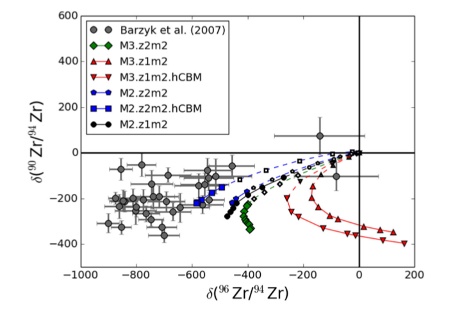
\includegraphics[width=\columnwidth]{figs/Zr94.png}
  \caption{This is a figure from \citet{zr} that contains their stellar model measurements of $\delta\left(\zirconium[96] / \zirconium[94]\right)$ as well as the SiC grain measurements from \citet{grain}. The models consistently over predict $\delta\left(\zirconium[96] / \zirconium[94]\right)$ which is from too much \zirconium[96] being produced in the He-flash PDCZ.} 
  \lFig{zr94}
\end{figure}

% Kippenhahn figure
\begin{figure}
  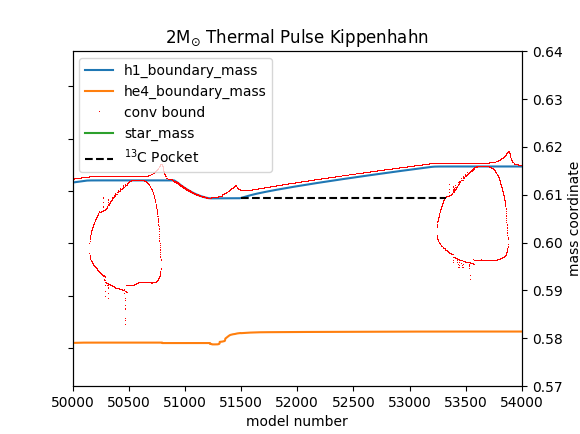
\includegraphics[width=\columnwidth]{figs/2M_Kippenhahn.png}
  \caption{Within the He intershell region, the \carbon[13] pocket forms and isotopic ratios are set by the \spr~(\Fig{zr_ratio13C}). It is then mixed and diluted in the He-flash pulse driven convection zone where temperatures get high enough to activate \neon[22]($\alpha,n$)\magnesium[25]. This shifts the isotopic ratios to those shown in \Figure{zr_ratioDil}.} 
  \lFig{kipp}
\end{figure}

\subsection{Neutron Density and Temperature}
\label{sec:neutron}

Within the PDCZ, the \neon[22] and \helium[4]/alpha particlse contribute a significant fraction of the mass contianed within it. There are a lot of alpha particles from the H-shell burning products from an earlier stage of evolution as well as the helium burning is not significant at this point (\Fig{kipp}). Once temperatures reach close to T$_{8} \approx 2.8$ within the PDCZ the \neon[22]($\alpha,n$)\magnesium[25] reaction is activated. This can be seen from the high neutron densities shown in \FigTwo{density}{neutron_sub}. When looking at a particular model number, the neutron density as a function of mass within the convective boundaries has a significant peak near the lower boundary. This is due to the \neon[22]($\alpha,n$)\magnesium[25] reaction being very sensitive to temperature and a huge portion of the reactions will take place at the bottom of the convection zone. The neutrons will then diffuse/mix throughout the convection zone allowing for the \spr~to take place. 

In \Fig{density}, the average neutron density steadily rises until the point where the convection zone reaches its maximum temperature and then slowly drops. This peak in the average neutron density is very short lived as it is only sustained for a few years. However, this will have an impact on the isotopic ratios of Zr as discussed in \Sect{branching}.

% neutron denisty time plot
\begin{figure}
  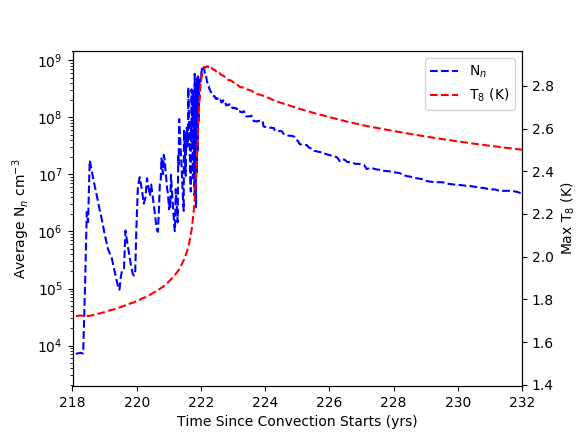
\includegraphics[width=\columnwidth]{figs/Neutron_Density_Time.png}
  \caption{This is a plot of the average neutron density and maximum temperature within the convection zone as a function of time. The temperature rises very rapidly and then slowly drops. This affects the average neutron density due to the sensitivity of the \neon[22]($\alpha,n$)\magnesium[25] reaction to temperature and can be seen clearly in this plot.} 
  \lFig{density}
\end{figure}

% sub time step neutron plots
\begin{figure}
   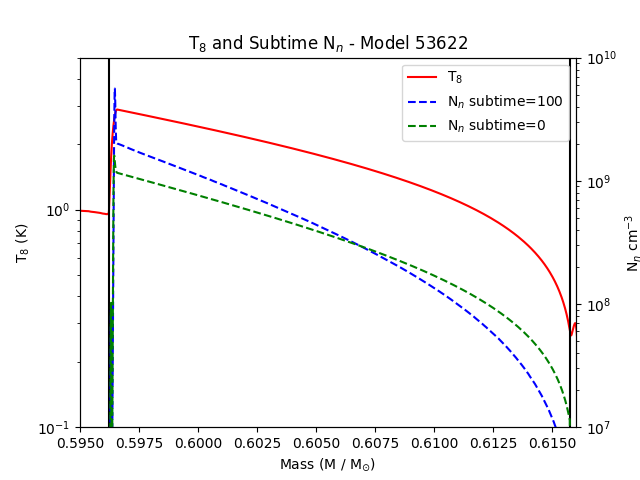
\includegraphics[width=1\columnwidth]{figs/T_Neutron_sub.png}
   \caption{These are profiles from the modified diffusion data (\Sect{diffusion}). The black vertical lines are where the convective boundaries are located. The temperature peaks very close to the lower convective boundary and the neutron density also peaks right at that point. There is a significant change in the neutron density when sub-time steps are used. This is attempting to resolve the \neon[22]($\alpha,n$)\magnesium[25] reaction at the lower convective boundary.}
   \lFig{neutron_sub}
\end{figure}

\subsection{Diffusion Coefficient Modifications}
\label{sec:diffusion}

The \MESA~models use the MLT and the diffusion equation to estimate how the mass fraction of isotopic species are transported and mixed throughout a convection zone. To calculate the change in mass fraction of a particular species at a particular mass coordinate in time, the stellar evolution codes solve the differential equation 
\begin{equation}
\frac{d\mathbf{X_{i}}}{dt} = \left. \frac{d\mathbf{X_{i}}}{dt} \right \rvert_{burn} + \left. \frac{d\mathbf{X_{i}}}{dt} \right \rvert_{mix}
\end{equation}

\noindent which contains the changes due to the possible reactions that the particular species can be involved in and the spatial diffusion of matter from the mixing in a convection zone. Using the diffusion formalism, this mixing term is given by
\begin{equation}
\left. \frac{d\mathbf{X_{i}}}{dt} \right \rvert_{mix} = \frac{\partial}{\partial m} [(4\pi r^{2} \rho)^{2} D(m) \frac{d\mathbf{X_{i}}}{dm}]
\label{eq:diffusion}
\end{equation} 

\noindent Where $D(m)$ is the diffusion coefficient at mass coordinate m. 

Using the MLT, the diffusion coefficient is given by
\begin{equation}
D = \frac{1}{3} v_{MLT} \alphaMLT H_{p}
\label{eq:diffusion_mlt}
\end{equation}

\noindent Where \alphaMLT$H_{p}$ is called the mixing length. By using the formalism of MLT, this diffusion would immediately go to zero at the Schwarzschild boundary (convective boundary) but overshoot is implemented and the diffusion coefficient is extended outside of the convective boundaries with use of \EQ{overshoot}. The Schwarzschild boundary is the mass coordinate where the Schwarzschild criterion, the condition in which the gas will be convectively unstable, is located. The Schwarzschild criterion is when the condition
\begin{equation}
\nablarad > \nablaad
\end{equation}

\noindent is satisfied. $\nablarad = \left(\dxdy{lnT}{lnP}\right)_{rad}$ is the gradient that the star would have if all of the energy is transported by radiation while $\nablaad = \left(\dxdy{lnT}{lnP}\right)_{ad}$ is the gradient the star would have if all of the energy was being transported by convection. 

The functionality of the MLT diffusion coefficient across the convection zone is similar to what is calculated from 3D hydrodynamic simulations. However, a main qualitative difference is that the diffusion coefficient begins to drop well before the convective boundary while the MLT diffusion coefficient will not. The reason behind this is that because the convective boundary is very stiff, an incompressible fluid would not be able to have a velocity profile that was nearly constant up to the boundary. It would need to slow down significantly as it got closer to that boundary as the fluid needs to disperse when it hits the wall with the condition that it cannot be compressed. A model for the diffusion coefficient that has been able to reproduce results from 3D hydro simulations is provided by \citep{4pi}. The formula for the diffusion coefficient is  
\begin{equation}
D_{hydro} = v_{MLT}min(\alphaMLT H_{p}, |r - r_{0}|)
\label{eq:Jones}
\end{equation} 

\noindent where $r_{0} = r_{SC} - f_{CBM}H_{p}^{SC}$ which are quantities that are evaluated at the Schwarzschild boundary. This does not make major changes to the functionality and magnitude of the diffusion coefficient except that it falls off quicker when approaching the convective boundaries. This can be seen in \Figure{diffusion}. With the temperature being highest at the lower convective boundary (\Fig{neutron_sub}) and with using \EQ{Jones} for the diffusion coefficient rather than \EQ{diffusion_mlt}, there would be less matter diffusing to the higher temperatures at the lower boundary. The possible nucleosynthetic consequences of this are discussed in \Sect{branching} and shown in \Sect{zr_zr}.

% diffusion plot
\begin{figure}
  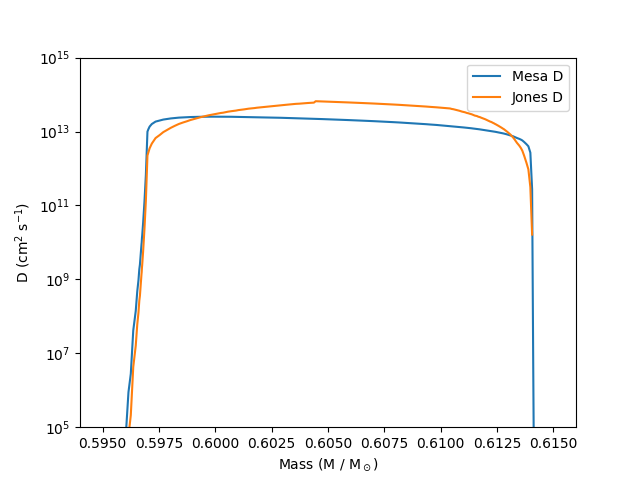
\includegraphics[width=\columnwidth]{figs/Diffusion_compare.png}
  \caption{The MLT diffusion coefficient has a more flat profile between the convective boundaries while the diffusion coefficient given by \citep{4pi} (\Eq{Jones}) is about an order of magnitude smaller at the convective boundaries.} 
  \lFig{diffusion}
\end{figure}

\subsection{\zirconium[95] and \iodine[128] Branching}
\label{sec:branching}

Within the \carbon[13] pocket, the reaction that causes the high neutron densities for the \spr~is \carbon[13]($\alpha,n$)\oxygen[16]. The neutron densities do not reach N$_{n} \approx 5\ee{8}\power{\centi\meter}{-3}$ that are required to open the \zirconium[95] branch \citep{zr}. This causes a situation in which there is production of \zirconium[94] from the \spr~but due to low neutron densities not as much \zirconium[96] is produced. This can be seen from the isotope mass fractions of Zr in \Fig{zr_ratio13C}. The \spr~path and \zirconium[95] branch can be seen in \Figure{zr95}

During the He-flash PDCZ temperatures get high enough for the \neon[22]($\alpha,n$)\magnesium[25] reaction to occur. Neutron densities can exceed the lower limit for the \zirconium[95] branching (\Fig{density}). This will shift the isotopic mass fractions of \zirconium[96] and \zirconium[94] to what is shown in \Figure{zr_ratioDil}. Their mass fractions dropped significantly due to the dilution of the \carbon[13] pocket into the PDCZ however the change in the ratio, log$_{10}$(\zirconium[96] / \zirconium[94]), went from -2.7 to -0.9. This is caused by the opening of the \zirconium[95] branch allowing for production of \zirconium[96]. This branch is only open for a very short amount of time as the neutron density is only larger than  $5\ee{8}\power{\centi\meter}{-3}$ for a few years (\Fig{density}) but its effects on the Zr isotopic ratios are significant. 

To compare with the measurements made by \citet{grain}, the isotopic ratios need to be represented into the per mil, $\delta$, form. For a given isotopic ratio, this is defined as
\begin{equation}
\delta\left(\zirconium[96] / \zirconium[94]\right) = [\left(\frac{\zirconium[96]}{\zirconium[94]} / \frac{\zirconium[96]_{\odot}}{\zirconium[94]_{\odot}}\right) - 1]\times 1000
\label{eq:mil}
\end{equation}

\noindent The comparison of $\delta\left(\zirconium[96] / \zirconium[94]\right)$ from the pre-solar grains measured by \citep{grain} and what stellar evolution models predict from \citep{zr} is in \Figure{zr94}.

The \iodine[128] isotope is unstable with a lifetime of only 25 minutes and it has two competing branches. These reactions are the $\beta^{-}$ decay, \iodine[128]($\beta^{-}$)\xenon[128], and the electron capture \iodine[128]($\beta^{+}$)\tellurium[128]. The electron capture rate is very sensitive to the temperature as well as the electron density \citep{reif}. \Figure{xe} shows all of the isotopes that play a role in the \iodine[128] branching. Within the He-flash PDCZ the temperature peaks very close to the lower convective boundary. With the convective time scale (\Sect{mppnp}) during the PDCZ being only a few hours, fresh \iodine[127] from the top of the convection zone will come to the bottom and can capture a neutron easily due to the very high neutron densities there. Because of the short half-life of \iodine[128], a significant portion of these will decay while being at the higher temperatures near the lower convective boundary. This will lead to a significant portion of the \iodine[128] to undergo \iodine[128]($\beta^{+}$)\tellurium[128] rather than \iodine[128]($\beta^{-}$)\xenon[128]. Since the \ppr~is not occurring within the He-flash PDCZ, the only production of \xenon[128] comes from the \iodine[128]($\beta^{-}$)\xenon[128] and there are losses of it from neutron captures. Because of this, the \xenon[128] / \xenon[130] ratio can be used as a tracer of what the dominating branch of \iodine[128] is.

% c13 pocket zr ratio
\begin{figure}
  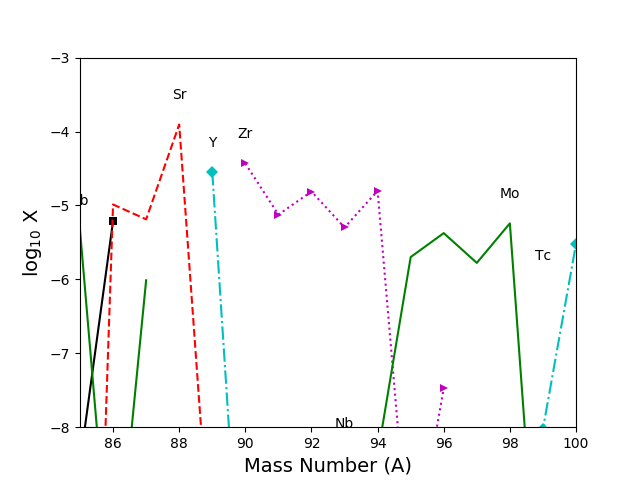
\includegraphics[width=\columnwidth]{figs/C13_Zr.png}
  \caption{These isotope ratios are averaged across the \carbon[13] pocket. Within the \carbon[13] pocket there is a significant amount of \zirconium[94] produced but almost no \zirconium[96]. This is due to the low neutron densities not opening the \zirconium[95] branch. The logarithm base 10 of the \zirconium[96] / \zirconium[94] ratio just before the \carbon[13] pocket is absorbed into the PDCZ is approximately -2.7.} 
  \lFig{zr_ratio13C}
\end{figure}

% Zr 95 branch
\begin{figure}
	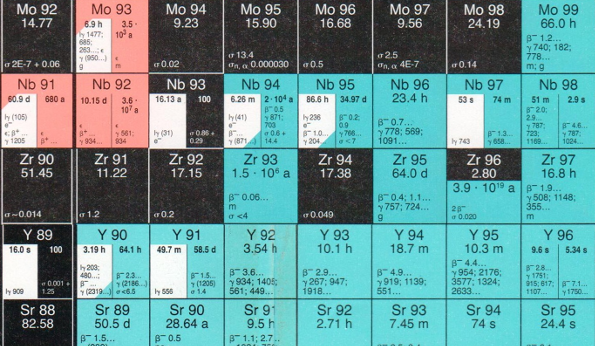
\includegraphics[width=\columnwidth]{figs/Zr95_branch.png}
    \caption{In order for there to be significant production of \zirconium[96] the neutron densities must be high enough such that the \zirconium[95] (half-life 64 days) does not all decay to \niobium[95]. The \zirconium[95] formed from the \zirconium[94]($n,\gamma$)\zirconium[95] reaction.}
    \lFig{zr95}
\end{figure}

% Zr ratio after pulse
\begin{figure}
  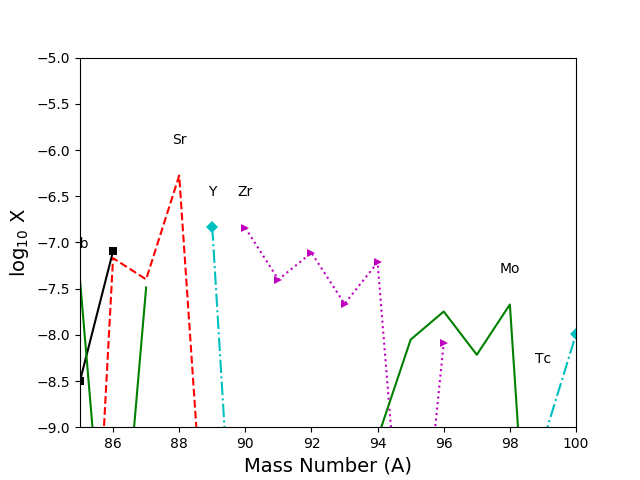
\includegraphics[width=\columnwidth]{figs/Pulse_Zr.png}
  \caption{These isotope ratios are averaged across the He-flash PDCZ. After the \carbon[13] pocket is mixed into the He-flash PDCZ, the temperatures get high enough for the \neon[22]($\alpha,n$)\magnesium[25] reaction. This provides high enough neutron densities to open the \zirconium[95] branch and boost the \zirconium[96]. The logarithm base 10 of the \zirconium[96] / \zirconium[94] ratio after the PDCZ is approximately -0.9.} 
  \lFig{zr_ratioDil}
\end{figure}

% Xe plot
\begin{figure}
	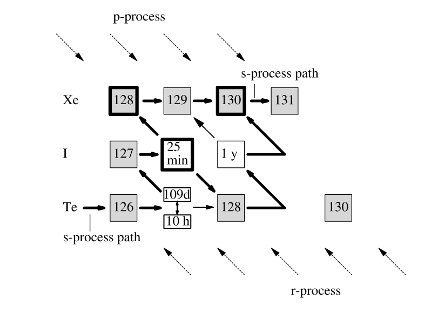
\includegraphics[width=\columnwidth]{figs/xe.png}
    \caption{The unstable isotope, \iodine[128], can either $\beta^{-}$ decay or capture an electron ($\beta^{+}$). The electron capture branching is very sensitive to the temperature. If it $\beta^{-}$ decays there will be production of \xenon[128]. If it captures an electron, it will decay to \tellurium[128] leading to no production of \xenon[128]. Loses of \xenon[128] are from neutron captures. This figure is from \citep{reif}.}
    \lFig{xe}
\end{figure}

\subsection{\mppnp~Post Processing}
\label{sec:mppnp}

The nucleosynthesis that was calculated with the \mppnp~code used a network of over 1000 isotopes and was limited by species that have a $\beta$ decay less than half a minute. Since only the \spr~can happen throughout this stars evolution up to the AGB, the neutron densities will not be high enough to have significant production of species with very short $\beta$ decay half lives. 

From using the \citet{models} models, the nucleosynthesis was already calculated for the 2\Msun, $Z=0.02$, throughout its entire evolution with the MLT diffusion coefficient. To calculate models with the diffusion coefficient from \EQ{Jones}, the H5 files that the \MESA~data was outputted to was modified. This was simply done with python and the \mppnp~code could be run normally but it would have the modified diffusion coefficient. 

Having a smaller diffusion coefficient at the lower convective boundary is expected to limit the amount of \neon[22] coming from the top of the convection to replenish what was lost from the \neon[22]($\alpha,n$)\magnesium[25] reaction. However, if a time step is so large that many convective turnover times have passed, this effect will not be observed. By default, \mppnp~will take a time step that the stellar evolution model (\MESA) took but evenly spaced sub-time steps between these can be taken. This is of course due to the fact that \mppnp~needs to utilize the thermodynamic quantities of the star at a particular point in time to compute the nucleosynthesis. In order to estimate how many sub-time steps are needed to resolve the convection, the convective time scale was calculated. With using MLT, the parcels of matter that convect have a velocity, v$_{MLT}$, and travel a mixing length on average. So the convective time scale is approximately
\begin{equation}
\tau_{conv.} \approx \frac{\alphaMLT}{\ensuremath{v_{\mathrm{MLT}}}}
\label{eq:tau}
\end{equation}

\noindent The convective time scale was calculated at every model number that had the He-flash PDCZ and was plotted with the time step that the \MESA~model took at that point. This is shown in \Figure{time_scale}. From this, if 100 sub-time steps are taken the convection can be resolved. The number of sub-time steps that were taken when \mppnp~was used with the 2\Msun, $Z=0.02$, \MESA~model was 100. 

Another thing to consider is the notion that the only way to know if a numerical result is something that is realistic with the models that were used to compute it, there needs to be numerical convergence. To achieve this, the resolution, or in this case number of time steps, needs to be increased to see if there are changes with the numerical results. If there are very minor changes, the solution that is found can be considered converged. In \Figure{neutron_sub}, the neutron density is measured with two different time steps and are plotted as a function of mass. The neutron density determined with 100 sub-time steps is about six times larger than the 0 sub-time step model at the mass coordinate of maximum temperature. This shows that the neutron densities were not converged with the zero sub-time steps for the modified diffusion coefficient models. If more time was spent on this work, a few more sub-time steps would have been chosen to check if this 100 sub-time solution is in fact converged.

% time scale plot
\begin{figure}
  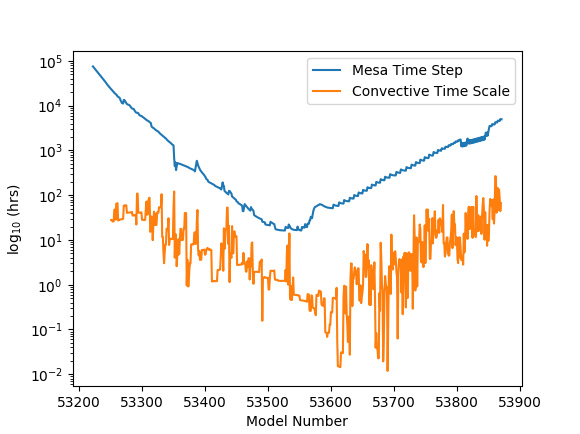
\includegraphics[width=\columnwidth]{figs/Time_scale.png}
  \caption{The time steps used by \MESA~are generally 100 times longer than the convective time scale at that model number. In order to resolve the impact of the hydro diffusion coefficient on the Zr isotopic ratios, the convection needs to be resolved. A sub-time step of 100 for \mppnp~allows for this.} 
  \lFig{time_scale}
\end{figure}

\section{Results}
\subsection{Effects on $\delta$(\zirconium[96] / \zirconium[94])}
\label{sec:zr_zr}

After running \mppnp~on the \MESA~H5 files with modified diffusion coefficients and 100 sub-time steps, the $\delta$(\zirconium[96] / \zirconium[94]) was calculated throughout the thermal pulse. This is shown in \Figure{zr_results}. Only the last 300 models were calculated due to the computational time needed. They were chosen such that the models with the highest temperatures, where the highest neutron densities would be, were computed. The values of $\delta$(\zirconium[96] / \zirconium[94]) that matter are after the He-flash PDCZ has finished. These are the isotopic ratios that will be mixed into the H envelope by the third dredge up. In \Figure{zr_results}, the $\delta$(\zirconium[96] / \zirconium[94]) is an average value across the maximum extent of the PDCZ for each model number. The $\delta$(\zirconium[96] / \zirconium[94]) from the zero sub-time steps modified diffusion model produced results that were not expected. However, it is likely that this model is not realistic as it had not been converged as the 100 sub-time step model provided entirely different results. These results are what had been expected as the number density of \zirconium[96] has decreased due to the decrease in neutron density. The $\delta$(\zirconium[96] / \zirconium[94]) from the 100 sub-time steps model is about 40 smaller than the original diffusion coefficient model. This is averaged across the entire PDCZ and so it is a significant difference for when this material gets mixed into the H envelope at the third dredge up. This effect would be amplified by the fact that this will occur for each thermal pulse in this model which there are 25 of.

% Zr results
\begin{figure}
   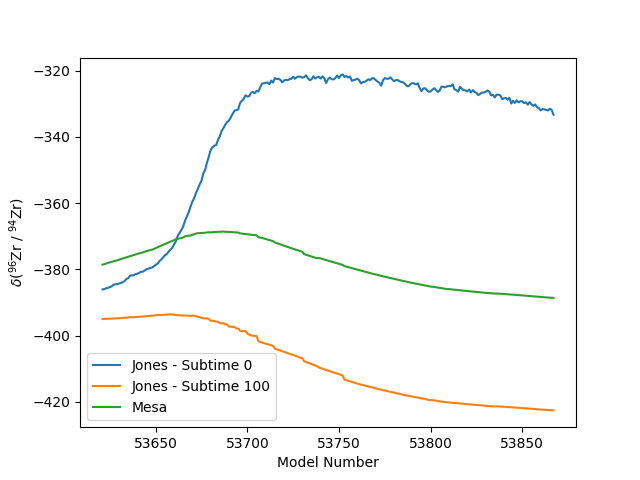
\includegraphics[width=1\columnwidth]{figs/JonesS1_zr.png}
   \caption{At the end of the convection zone (the last model number), the $\delta\left(\zirconium[96] / \zirconium[94]\right)$ from the 100 sub-time step model with the modified diffusion coefficient is significantly lower than the same quantity from the original nucleosynthesis results. The no sub-time step model shows very unintuitive results.}
   \lFig{zr_results}
\end{figure}

\subsection{The \xenon[128] / \xenon[130] Ratio}

With the same data as what was used in the previous section, a similar analysis was conducted for the \xenon[128] / \xenon[130] ratio. They were averaged results across the maximum extent across the PDCZ and they are shown in \Figure{xe_results}. At the end of the PDCZ, the \xenon[128] / \xenon[130] ratio for the 100 sub-time step model did not change significantly from the baseline models. The expectation was that the \iodine[128]($\beta^{+}$)\tellurium[128] reaction would occur less frequently as there would be less of it at the highest temperatures in the PDCZ. One possibility for the insignificant change is that this reaction had not been resolved with the time steps chosen. The half-life of \iodine[128] is only 25 minutes while the time steps that were used were not smaller than a few hours (\Fig{time_scale}).

% xenon results
\begin{figure}
   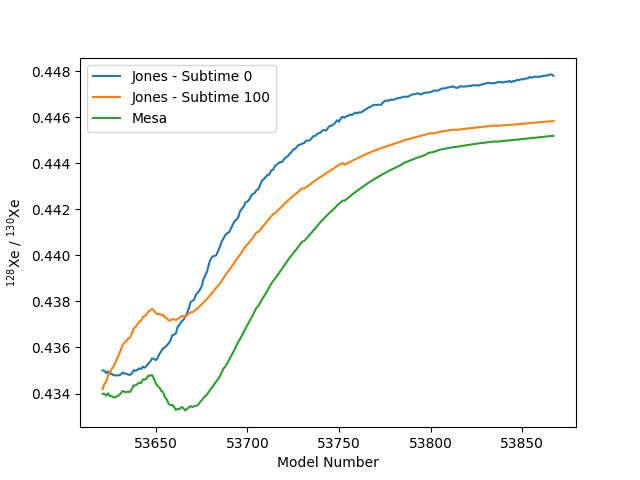
\includegraphics[width=1\columnwidth]{figs/JonesS1_xe2.png}
   \caption{At the end of the convection zone (the last model number), the \xenon[128] / \xenon[130] ratio does not change much. It appears as though the \iodine[128] branch is not affected by the changes to the diffusion coefficient.}
   \lFig{xe_results}
\end{figure}

\section{Conclusions}

The 2\Msun,$Z=0.02$, stellar model from \citet{models} was modified by changing the diffusion coefficients to the model stated in \citet{4pi}, \EQ{Jones}. The post-processing nucleosynthesis was computed with \mppnp~and 100 sub-time steps were used to resolve the convection. The  $\delta$(\zirconium[96] / \zirconium[94]) and \xenon[128] / \xenon[130] were averaged across the maximum extent of the PDCZ. These are the isotopic ratios that would be mixed into the H envelope from the third dredge up and can be measured in the SiC grains that would form when this mass is lost from stellar winds during the AGB phase.

The \xenon[128] / \xenon[130] ratio that was measured with the modified diffusion coefficients and 100 sub-time steps was not significantly different from the baseline \MESA~model, \mppnp~post processed predictions. This may be due to not resolving the \iodine[128] branching as the sub-time steps amounted to a few hours while its half-life is only 25 minutes. 

The $\delta$(\zirconium[96] / \zirconium[94]) measured cannot directly be compared with results from \citep{zr} as theirs are measured after being mixed into the H envelope. There is also the fact that the results from this work are only due to one PDCZ, the 24$^{th}$, and the feedback effects from this happening many times is not taken into account. However, the results do state that the $\delta$(\zirconium[96] / \zirconium[94]) from the modified diffusion coefficient is less than the other models which would better match the observations found in \citep{grain}. To fully quantify the effects the modified diffusion coefficient would have on the Zr isotopic ratios, this would need to be applied to all thermal pulses throughout the AGB phase. These results are based on the assumption that this solution has converged but no test has definitively shown this.

 

\section*{Acknowledgements}

I would like to acknowledge the suggestions and input that Falk Herwig had throughout my undertaking of this project. His guidance allowed for the completion of this project in the limited time frame that I had.

%%%%%%%%%%%%%%%%%%%%%%%%%%%%%%%%%%%%%%%%%%%%%%%%%%

%%%%%%%%%%%%%%%%%%%% REFERENCES %%%%%%%%%%%%%%%%%%

% The best way to enter references is to use BibTeX:

\bibliographystyle{mnras}
\bibliography{paper.bib} % if your bibtex file is
                                             % called example.bib



%%%%%%%%%%%%%%%%%%%%%%%%%%%%%%%%%%%%%%%%%%%%%%%%%%

%%%%%%%%%%%%%%%%% APPENDICES %%%%%%%%%%%%%%%%%%%%%


%%%%%%%%%%%%%%%%%%%%%%%%%%%%%%%%%%%%%%%%%%%%%%%%%%


% Don't change these lines
\bsp	% typesetting comment
\label{lastpage}
\end{document}

% End of mnras_template.tex
